\documentclass[10pt]{article}

% amsmath package, useful for mathematical formulas
\usepackage{amsmath}
% amssymb package, useful for mathematical symbols
\usepackage{amssymb}
% graphicx package, useful for including eps and pdf graphics
% include graphics with the command \includegraphics
\usepackage{graphicx}
\usepackage{color}
\pdfpagebox5
\usepackage{pgfplots}
\usepgfplotslibrary{dateplot}

\newcommand{\Rdp}{\ensuremath{R_{\Delta\%}}}
\newcommand{\fR}{\ensuremath{f_R}}


\begin{document}

\pgfplotscreateplotcyclelist{pontvariety}{%
{blue},
{green},
{red},
{orange}
}

\newcommand{\fn}[1]{#1.csv}
%\newcommand{\fn}[1]{validation/pontailler1999/coppice/#1.csv}

\pgfplotstableread[col sep=comma]{ws.csv}\ws
%\pgfplotstableread[col sep=comma]{validation/pontailler1999/ws.csv}\ws

\newcommand{\plotvarieties}[1]{
    \pgfplotsset{cycle list name={pontvariety},cycle list shift=#1}
    \addplot table [x=date, y=Beaupre] {\ws};
    \addplot table [x=date, y=Raspalje]{\ws};
    \addplot table [x=date, y=Pauley] {\ws};
    \addplot table [x=date, y=Robusta] {\ws};
}

\begin{tikzpicture}
  \begin{axis}[
    width=\linewidth,
    height=3in,
    date coordinates in=x,
    xmin={1987-01-15},
    xmax={1997-12-15},
    xtick={
      {1987-12-15},
      {1988-12-15},
      {1989-12-15},
      {1990-12-15},
      {1991-12-15},
      {1992-12-15},
      {1993-12-15},
      {1994-12-15},
      {1995-12-15},
      {1996-12-15},
      {1997-12-15}
    },
    x tick label style={rotate=45, anchor=east},
    xticklabel={\year-\month},
    ylabel=Stem Biomass (Mg ha-1),
    legend entries={Beaupre,Pauley-Fritzi,Raspalje,Robusta},
    legend style={
       at={(0.5,1.0)},anchor=south,yshift=2pt,legend columns=-1
     },
     table/col sep=comma,
     cycle list name = pontvariety,
     no markers,
     every axis plot/.append style={line width=1pt},
     every mark/.append style={solid}
    ]
    \addplot+[only marks] table [x=date, y=Beaupre] {\ws};
%    \addplot+[boxplot={data={y}} ] table [x=date,y=Beaupre} {\ws};
    \addplot+[only marks] table [x=date, y=Raspalje]{\ws};
    \addplot+[only marks] table [x=date, y=Pauley] {\ws};
    \addplot+[only marks] table [x=date, y=Robusta] {\ws};
%    \plotvarieties{-5}
    \pgfplotsset{cycle list shift=-4}
    \addplot table [x=date, y=WS] {\fn{pont-beaupre-best}};
    \addplot table [x=date, y=WS] {\fn{pont-fritzi-best}};
    \addplot table [x=date, y=WS] {\fn{pont-raspalje-best}};
    \addplot table [x=date, y=WS] {\fn{pont-robusta-best}};
    \addplot+[color=black] table [x=date, y=WS] {\fn{pont-raspalje}};

  \end{axis}
\end{tikzpicture}

\begin{figure}[p]
  \centering
  
\pgfplotsset{
      no markers,
      width=0.5\linewidth,
      height=0.25\linewidth,
      every axis plot/.append style={line width=1pt},
      date coordinates in=x,
      xmin={2017-03-15},
      xmax={2019-10-15},
      xtick={
      2017-06-15,2017-09-15,2017-12-15,
      2018-03-15,2018-06-15,2018-09-15,2018-12-15,
      2019-03-15,2019-06-15,2019-09-15},
      xticklabels=\empty,
}
  \begin{tikzpicture}
    \begin{axis}[
      name=ws11,
      ymin=0,ymax=80,
      ytick={20,40,60},
      yticklabels={20,40,60},
      ylabel=Stem~$\frac{T}{ha}$,
      legend entries={$\Rdp=0.001$,$\Rdp=0.01$,$\Rdp=0.1$,$\Rdp=0.5$,$\Rdp=1$},
      legend style={
        at={(1.0,1.0)},anchor=south,legend columns=-1,yshift=2pt}
      ]
      \node at (axis cs:{2018-02-15},50) {Nov};
      \addplot+[color=red] table [x=date, y=m11f0.001, col sep=comma] {hart12coppice-coppice-ws.csv};
      \addplot+[color=orange] table [x=date, y=m11f0.01, col sep=comma] {hart12coppice-coppice-ws.csv};
      \addplot+[color=yellow] table [x=date, y=m11f0.1, col sep=comma] {hart12coppice-coppice-ws.csv};
      \addplot+[color=green] table [x=date, y=m11f0.5, col sep=comma] {hart12coppice-coppice-ws.csv};
      \addplot+[color=blue] table [x=date, y=m11f1, col sep=comma] {hart12coppice-coppice-ws.csv};
    \end{axis}
    \begin{axis}[
      name=wf11,
      ylabel=Foliage,
      at={(ws11.below south west)},yshift=5pt,
      anchor=north west,
      ymin=0,ymax=30,
      ytick={10,20},
      yticklabels={10,20},
      ]
      \addplot+[color=red] table [x=date, y=m11f0.001, col sep=comma] {hart12coppice-coppice-wf.csv};
      \addplot+[color=orange] table [x=date, y=m11f0.01, col sep=comma] {hart12coppice-coppice-wf.csv};
      \addplot+[color=yellow] table [x=date, y=m11f0.1, col sep=comma] {hart12coppice-coppice-wf.csv};
      \addplot+[color=green] table [x=date, y=m11f0.5, col sep=comma] {hart12coppice-coppice-wf.csv};
      \addplot+[color=blue] table [x=date, y=m11f1, col sep=comma] {hart12coppice-coppice-wf.csv};
    \end{axis}

    \begin{axis}[
      name=wr11,
      at={(wf11.below south west)},yshift=5pt,
      anchor=north west,
      x tick label style={rotate=45, anchor=east},
      xticklabels={
      Y3-06,Y3-09,Y3-12,
      Y4-03,Y4-06,Y4-09,Y4-12,
      Y5-03,Y5-06,Y5-09},
      ymin=5,ymax=30,
      ytick={10,20},
      yticklabels={10,20},
      ylabel=Root,
      ]
      \addplot+[color=red] table [x=date, y=m11f0.001, col sep=comma] {hart12coppice-coppice-wr.csv};
      \addplot+[color=orange] table [x=date, y=m11f0.01, col sep=comma] {hart12coppice-coppice-wr.csv};
      \addplot+[color=yellow] table [x=date, y=m11f0.1, col sep=comma] {hart12coppice-coppice-wr.csv};
      \addplot+[color=green] table [x=date, y=m11f0.5, col sep=comma] {hart12coppice-coppice-wr.csv};
      \addplot+[color=blue] table [x=date, y=m11f1, col sep=comma] {hart12coppice-coppice-wr.csv};
    \end{axis}

  \end{tikzpicture}

  \caption{ { \bf Coppice regrowth model results for various levels of Root
      contribution \Rdp.}  Y-axis is the dry mass of each component of the
    plantation, in terms of $\frac{T}{ha}$. $\Rdp=100$ and $\fR=1$.}
  \label{fig:rdp}
\end{figure}

\begin{figure}
  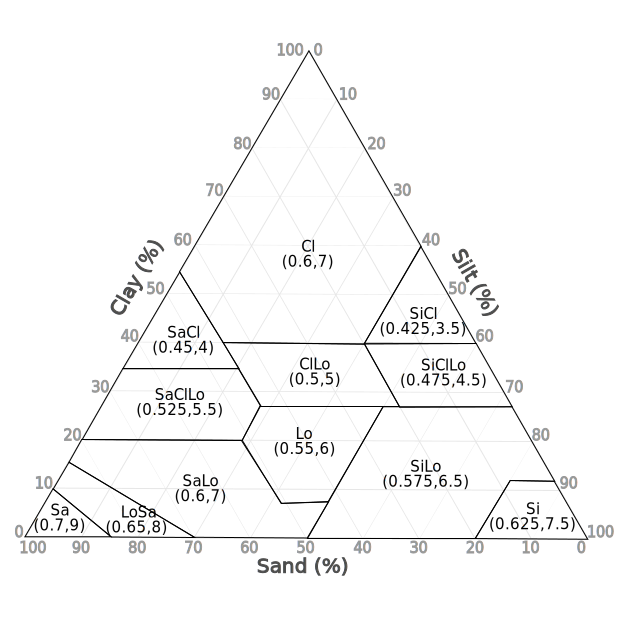
\includegraphics[width=0.45\linewidth]{../soil_triangle}
    \begin{tikzpicture}
    \begin{axis}[
      name=fsw,
      xmin=0,xmax=1,
      xtick={0,.2,.4,.6,.8,1},
      xticklabels={0,.2,.4,.6,.8,1},
      xlabel=$\acs{AWS}/\acs{maxAWS}$,
      ymin=0,ymax=1,
      ytick={0,.2,.4,.6,.8,1},
      yticklabels={0,.2,.4,.6,.8,1},
      ylabel=$\acs{fSW}$,
      no markers,
      width=0.45\linewidth,
      height=0.45\linewidth,
      every axis plot/.append style={line width=1pt},
      legend entries={sand,clay,silt},
      legend style={
        at={(0.5,1.0)},anchor=south,legend columns=-1,yshift=2pt}
      ]
      \addplot+[color=red] table [x=awsp, y=Sand, col sep=comma] {soil-fsw.csv};
      \addplot+[color=orange] table [x=awsp, y=Clay, col sep=comma] {soil-fsw.csv};
      \addplot+[color=green] table [x=awsp, y=Silt, col sep=comma] {soil-fsw.csv};
    \end{axis}
  \end{tikzpicture}

  \caption{\acs{swc} and \acs{swp} as determined by soil composition.  Included is a graph for the function  }
\end{document}
